
\section{Algorithms}

\frame{
	\frametitle{Notation}
	
	Using a hypergraph view
	\begin{itemize}
		\item $u, v, s$ are nodes
		\item $e$ is an edge\\
		\item $\head(e)$ is a node
		\item $\tail(e)$ is a sequence of nodes
		\item if $u \in \tail(e)$ and $v \in \tail(e)$, $u$ and $v$ are siblings 
		\item Backward-star: $BS(u)$ is the set of edges incoming to $u$\\
		$u$ is the head of the edge
		\item Forward-star: $FS(u)$ is the set of edges outgoing from $u$\\
		$u$ is in the tail of the edge
		\item $w(e)$ is the weight of an edge		
	\end{itemize}


}

\frame{
	\frametitle{Inside}
	
	The \textsc{Inside} recursion 
	
	\begin{equation}
	I(v) = 
	\begin{cases}
		 \bar{1} & \text{if } BS(v) = \emptyset\\
		 {\displaystyle \bigoplus_{e \in BS(v)}} \omega(e) \otimes {\displaystyle\bigotimes_{u \in \tail(e)}} I(u) & \text{otherwise}
	\end{cases}
	\end{equation}
	
	
	\hfill\alert{For acyclic hypergraphs} 
		
}


\frame{
	\frametitle{Outside}
	
	The \textsc{Outside} recursion 
	
	\begin{equation}
	O(v) = 
	\begin{cases}
		 \bar{1} & \text{if } FS(v) = \emptyset \\
		 \displaystyle \bigoplus_{e \in FS(v)} \omega(e) \otimes O(\head(e)) \otimes  {\displaystyle\bigotimes_{s \in tail(e)\setminus \{v\}}} I(s) & \text{otherwise}
	\end{cases}
	\end{equation}
	
	
	\hfill\alert{For acyclic hypergraphs} 
		
}

\frame[plain]{
	\frametitle{Topsort}
	
	
\begin{algorithmic}[1]\small
\Function{TopSort}{$G = \angbrack{V, \angbrack{E, w}}$}%$G = \angbrack{\Sigma, V, \angbrack{S, \sigma}, \angbrack{R, 	
	\State $S = \{v \in V: BS(v) = \emptyset \}$ \Comment{nodes with no dependencies}\label{line:nodep}
%	\State $D =\{q \mapsto \text{children}(q): q \in V\}$ \Comment{dependencies of each node}
	\State $D =\{v \mapsto \{u: \exists e \in BS(v) \wedge u \in \tail(e)\}: v \in V\}$ 
	\State \Comment{a node depends on all of its children}\label{line:yesdep}	
	\State $L = \angbrack{}$ \Comment{top-sorted nodes}
	\While{$S \neq \emptyset$}
		\State $u \la \text{pop}(S)$ \Comment{remove and return a node from $S$}
		%\State $q \in S, S \la S\setminus \{q\}$
		\State $L \la L + \angbrack{u}$ \Comment{append $u$ to $L$}
		\For{$e$ in $FS(u)$} \Comment{outgoing edges from $u$}
			\State $v \la \head(e)$ \Comment{parent of $u$ in $e$}
			\State $D(v) \la D(v)\setminus \{u\}$ \Comment{remove $u$ from $D(v)$}
			%\State remove $q$ from $D(p)$
			\If{$D(v) == \emptyset$} \Comment{$v$'s dependencies have been sorted}
				\State $S \la S \cup \{v\}$ \label{line:determined}
			\EndIf
		\EndFor
	\EndWhile
	\State \Return $L$
\EndFunction
\end{algorithmic}

}

\frame[plain]{
	\frametitle{Inside}
	
	\begin{algorithmic}[1]\small
\Function{Inside}{$G = \angbrack{V, \angbrack{E, w}}$} %$G = \angbrack{\Sigma, V, \angbrack{S, \sigma}, \angbrack{R, \nu}}$}
\For{$v$ in \Call{TopSort}{$G$}} \Comment{visit nodes bottom-up} 
	\If{$BS(v) == \emptyset$} 
		\State $I[v] \la \bar{1}$ \Comment{leaves}
	\Else
		\State $I[v] \la \bar{0}$
		\For{$e \in BS(v)$} %\Comment{total inside weight of an incoming edge}
			\State $k \la w(e)$ \Comment{include the edge's own weight}
			\For{$u$ in $\tail(e)$} %\Comment{this is the tail of the edge}
				\State $k \la k \otimes I[u]$ 
			\EndFor
			\State $I[v] \la I[v] \oplus k$ \Comment{accumulate for each edge}
		\EndFor
	\EndIf
\EndFor
\State \Return $I$
\EndFunction
\end{algorithmic}

}

\frame[plain]{
	\frametitle{Outside}
	
	\begin{algorithmic}[1]\small
\Function{Outside}{$G = \angbrack{V, \angbrack{E, w}}, I, \text{root}$}
	\State $O[v] \la \bar{0} \textbf{ for } v \in V $
\State $O[\text{root}] \la \bar{1}$ \Comment{this is the goal node}
\For{$v$ in \textsc{reverse}(\Call{TopSort}{$G$})} \Comment{visit nodes top-down}
	\For{$e \in BS(v)$} \Comment{$q$'s incoming edges}
		\For{$u \in \tail(e)$} \Comment{children of $v$ in $e$}
			\State $k \la w(e) \otimes O[v]$ 
			\For{$s$ in $\tail(e)$} \Comment{siblings of $u$ in $e$}
				\If{$u \neq s$} \Comment{$u$ itself is excluded}
					\State $k \la k \otimes I[s]$ %\Comment{incorporate inside weights surrounding $r$}
				\EndIf
			\EndFor
			\State $O[u] \la O[u] \oplus k$ \Comment{accumulate it for $u$}
		\EndFor
	\EndFor
\EndFor
\State \Return $O$
\EndFunction
\end{algorithmic}

}

\frame[plain]{
	\frametitle{Expected features}
	
	\begin{algorithmic}[1]\small
\Function{ExpectedFeatures}{$G = \angbrack{V, \angbrack{E, w}}, I, O, \phi$}
	\State $\bar{\phi} \la 0$
\For{$e \in E$} \Comment{these are edges}
	\State $k \la  O[\head(e)]$
	\For{$u$ in $\tail(e)$}
		\State $k \la k \otimes I[u]$
	\EndFor
	\State $\bar{\phi} \la \bar{\phi} + k \phi(e)$
\EndFor
\State \Return $\bar{\phi}$ \Comment{expected feature vector}
\EndFunction
\end{algorithmic}
}


\frame{
	\frametitle{Traversals}
	
	Viterbi derivation
	\begin{enumerate}
		\item start from the goal (root) 
		\item recursively rewrite every symbol $v$ by solving
		$$e^\star = \argmax_{e \in BS(v)} w(e)\bigotimes_{u \in \tail(e)} I(u)$$
	\end{enumerate}
	
	\pause
	Sampling
	\begin{enumerate}
		\item start from the goal (root)
		\item recursively rewrite every symbol $v$ by solving
		\[
		E \sim P(e|v) = 
	\begin{cases}
		 \bar{0} & \text{if } e \not\in BS(v)\\
		 \frac{w(e)\bigotimes_{u \in \tail(e)} I(u)}{I(v)} & \text{otherwise}
	\end{cases}
		\]
	\end{enumerate}
}

\frame{
	\frametitle{Viterbi}
	
	Use Inside computed in the Max-Times semiring!
	
	\only<1>{
	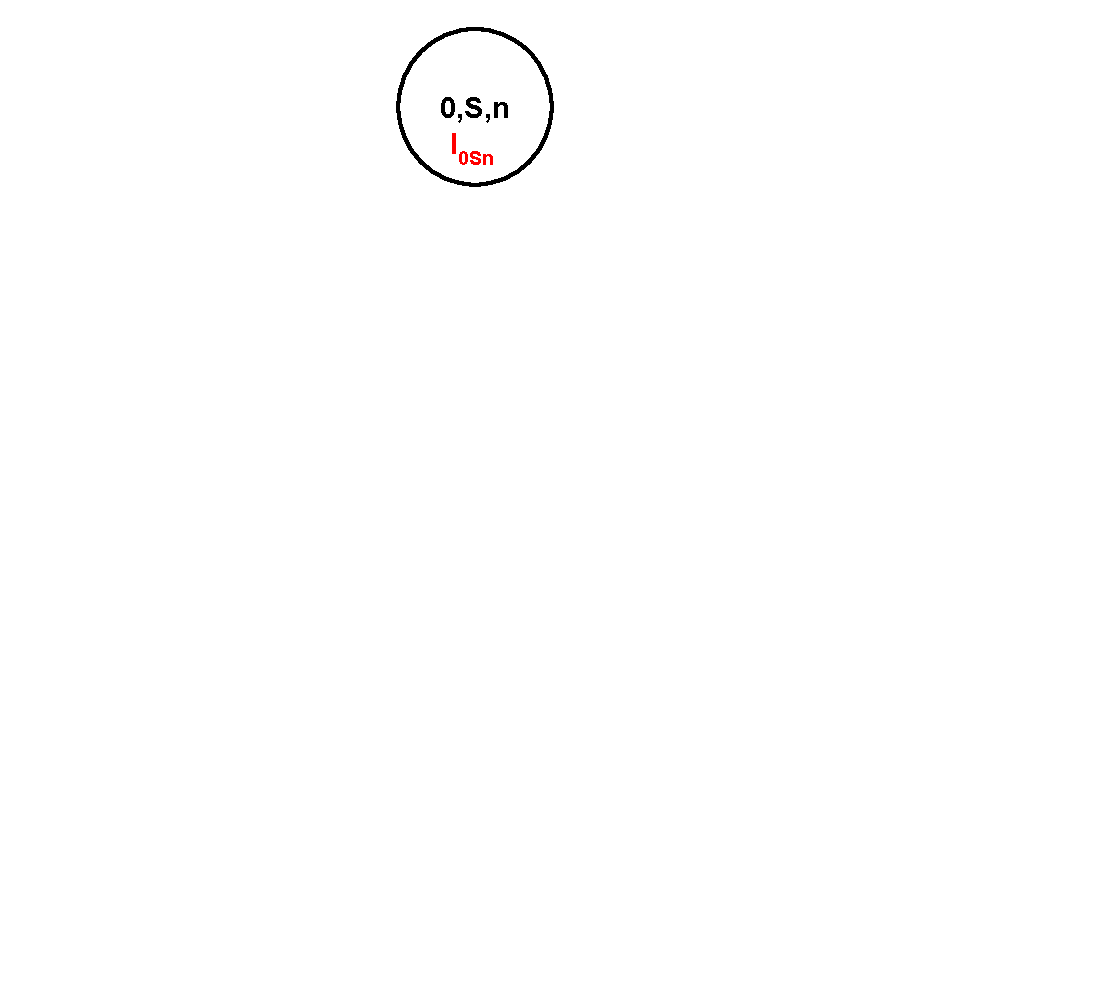
\includegraphics[scale=0.3]{img/viterbi0}
	}
	\only<2>{
	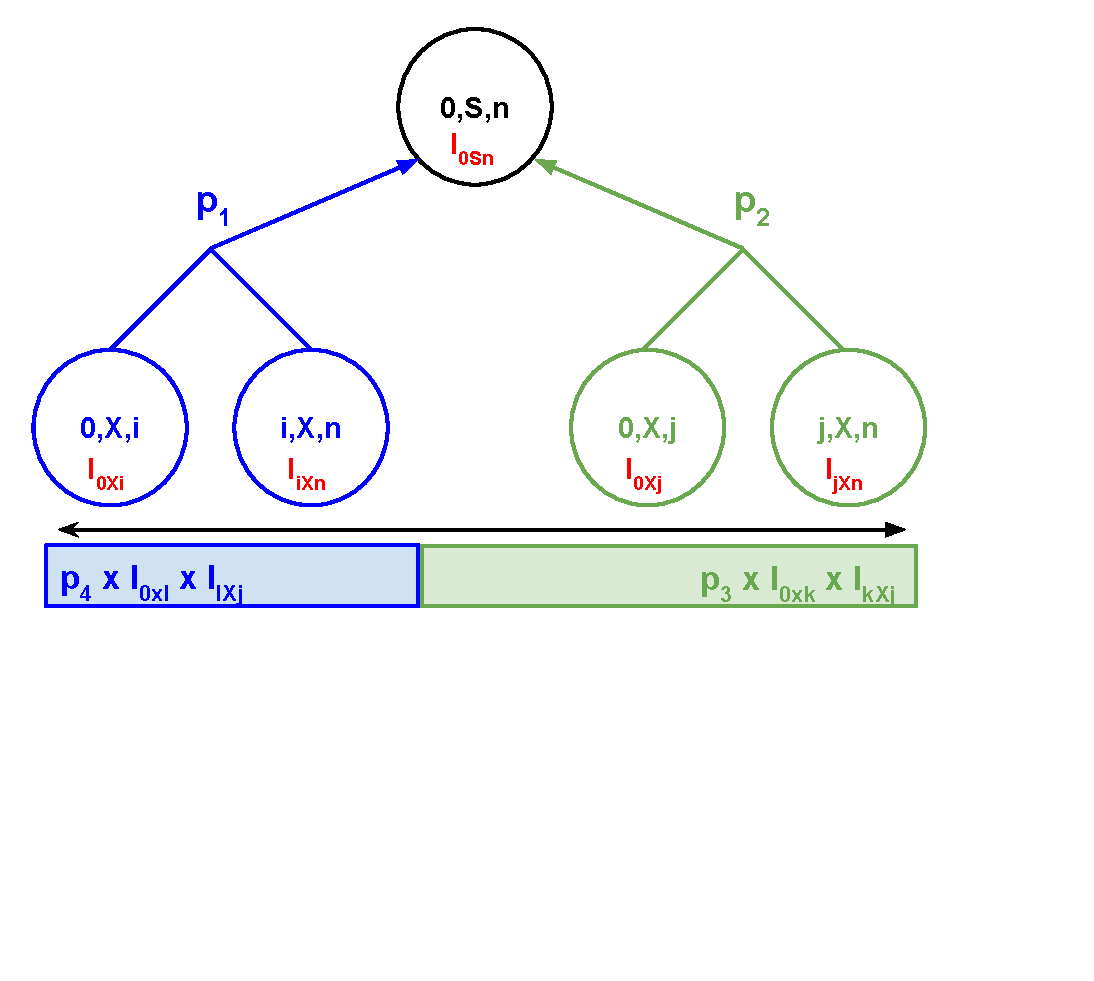
\includegraphics[scale=0.3]{img/viterbi1}
	}
	\only<3>{
	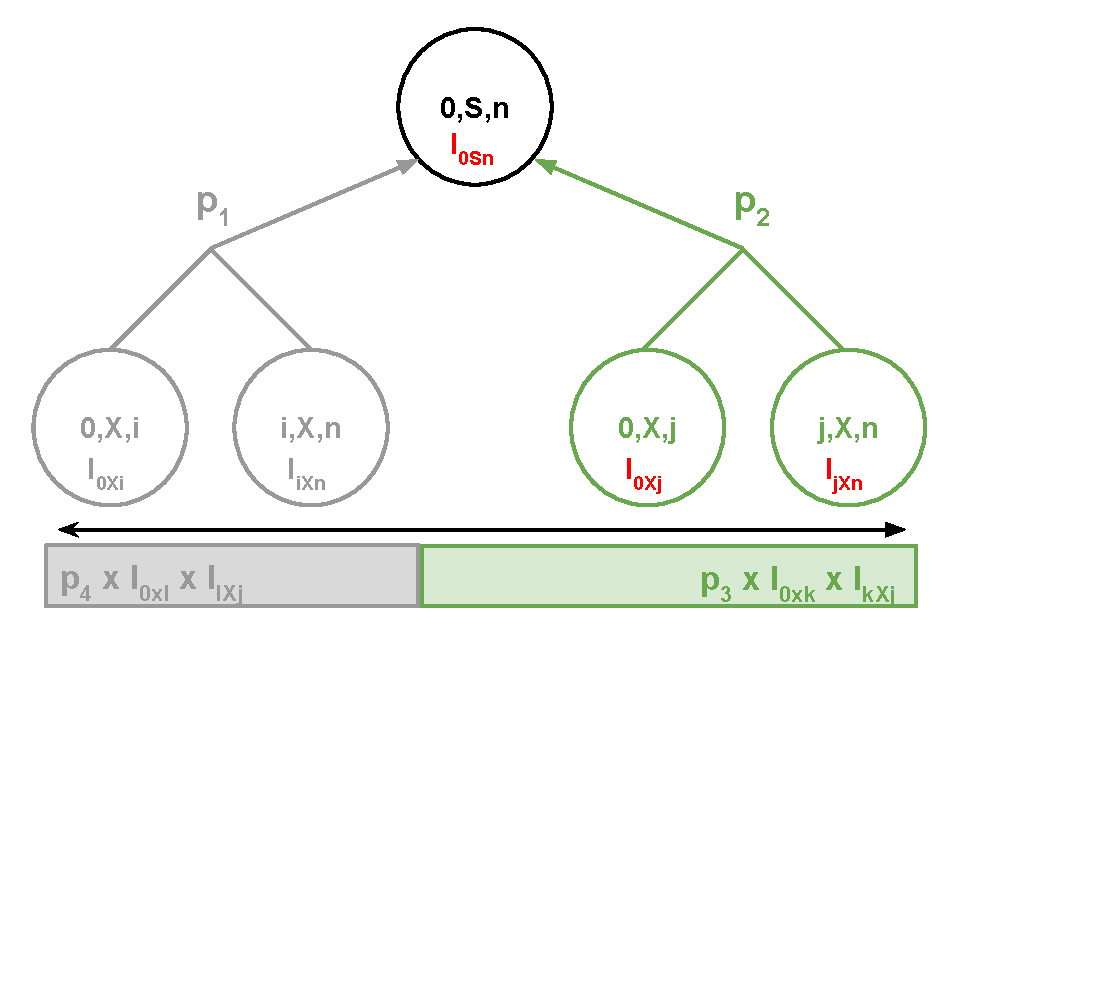
\includegraphics[scale=0.3]{img/viterbi2}
	}
	\only<4>{
	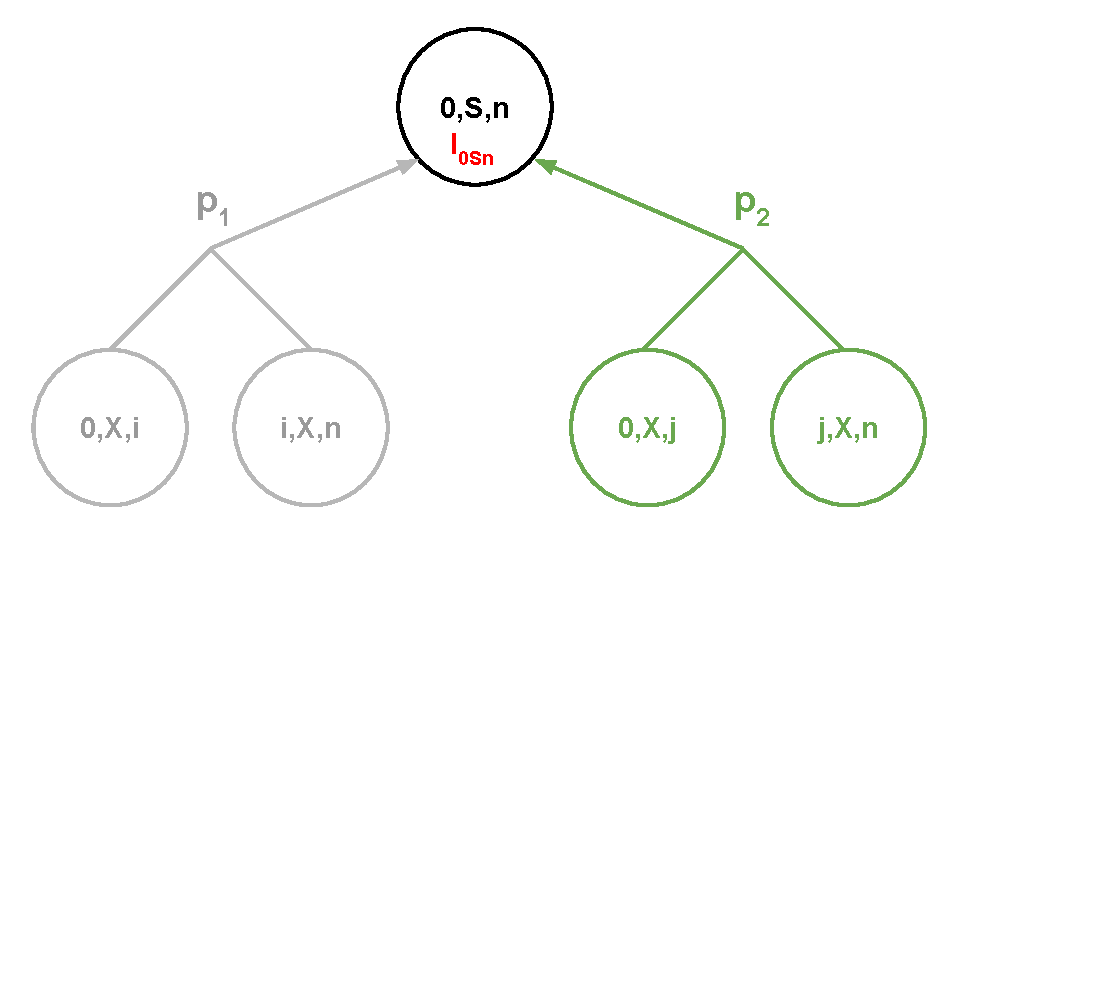
\includegraphics[scale=0.3]{img/viterbi3}
	}
	\only<5>{
	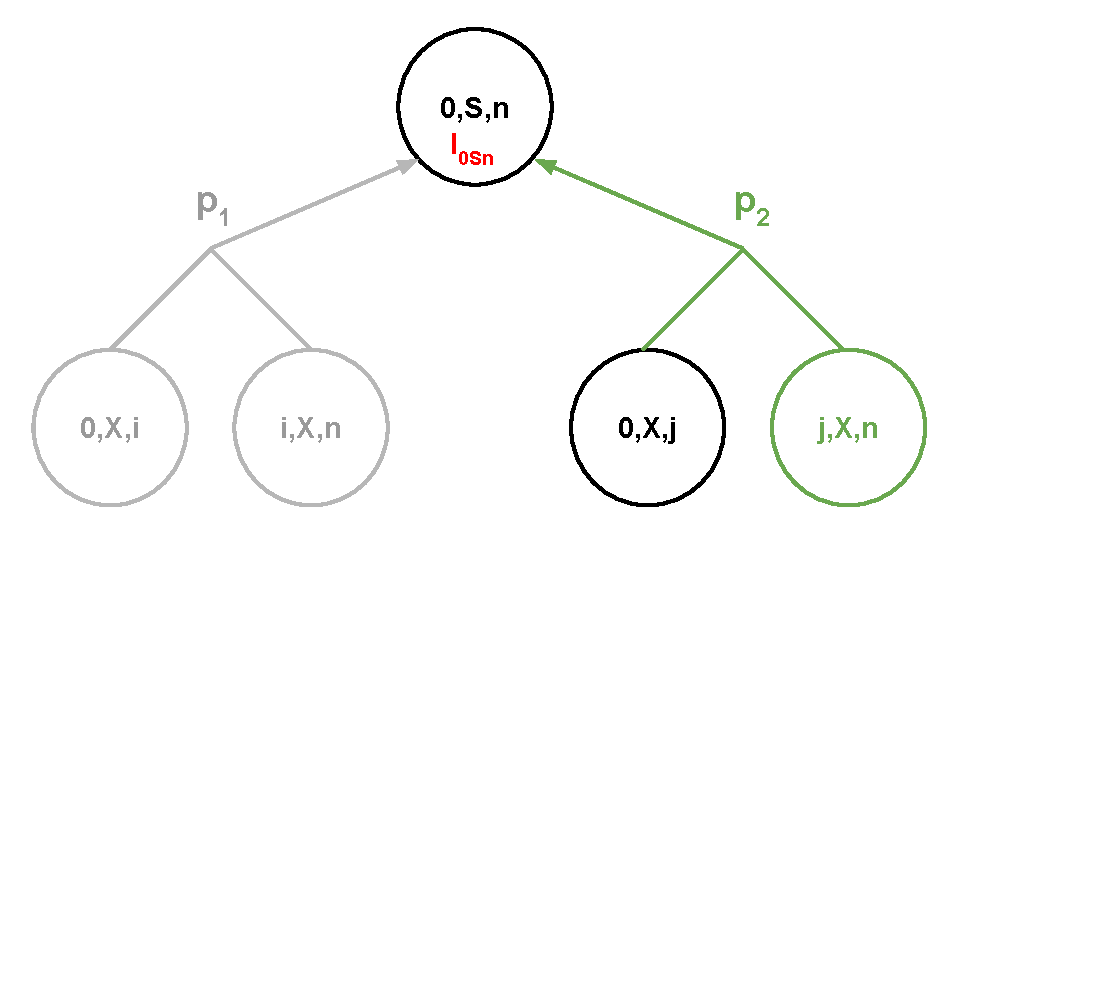
\includegraphics[scale=0.3]{img/viterbi4}
	}
	\only<6>{
	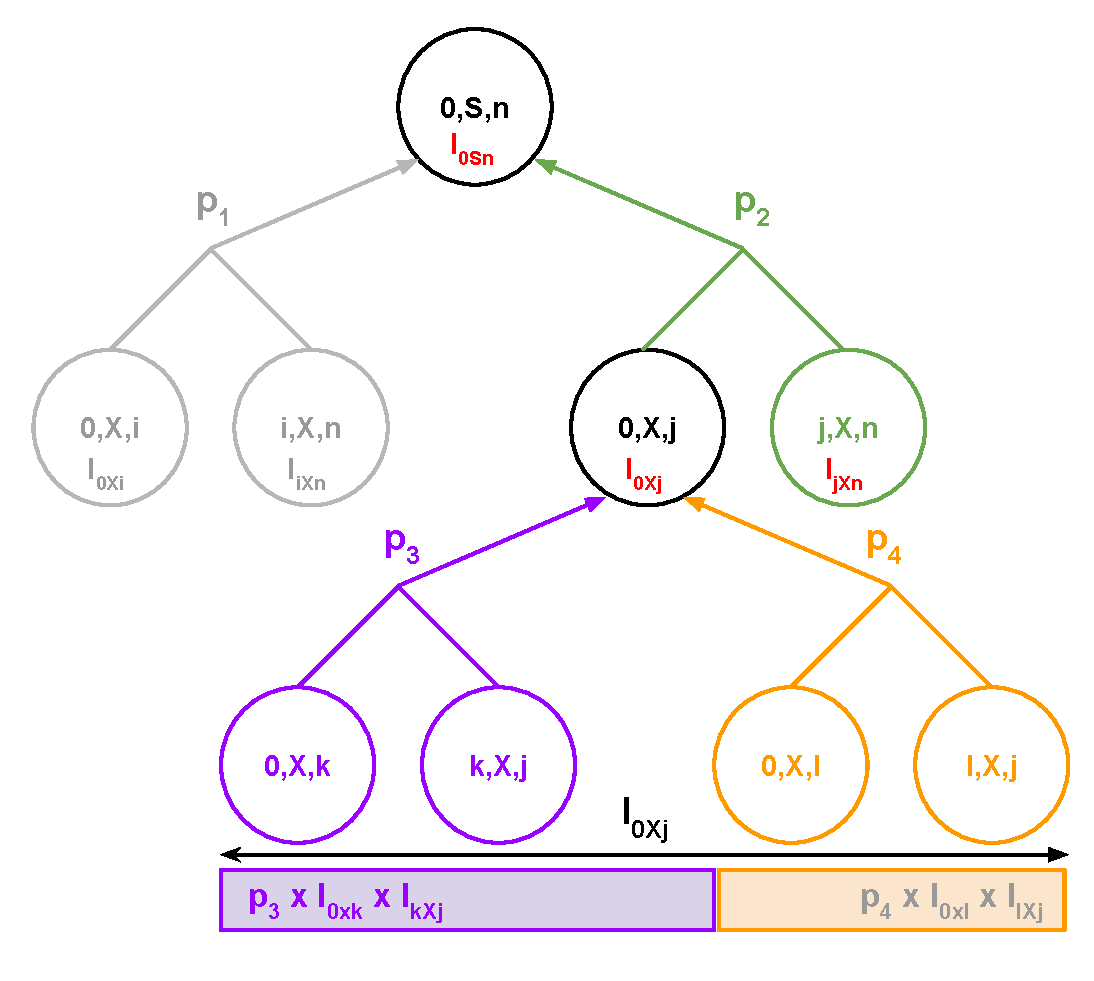
\includegraphics[scale=0.3]{img/viterbi5}
	}
	\only<7>{
	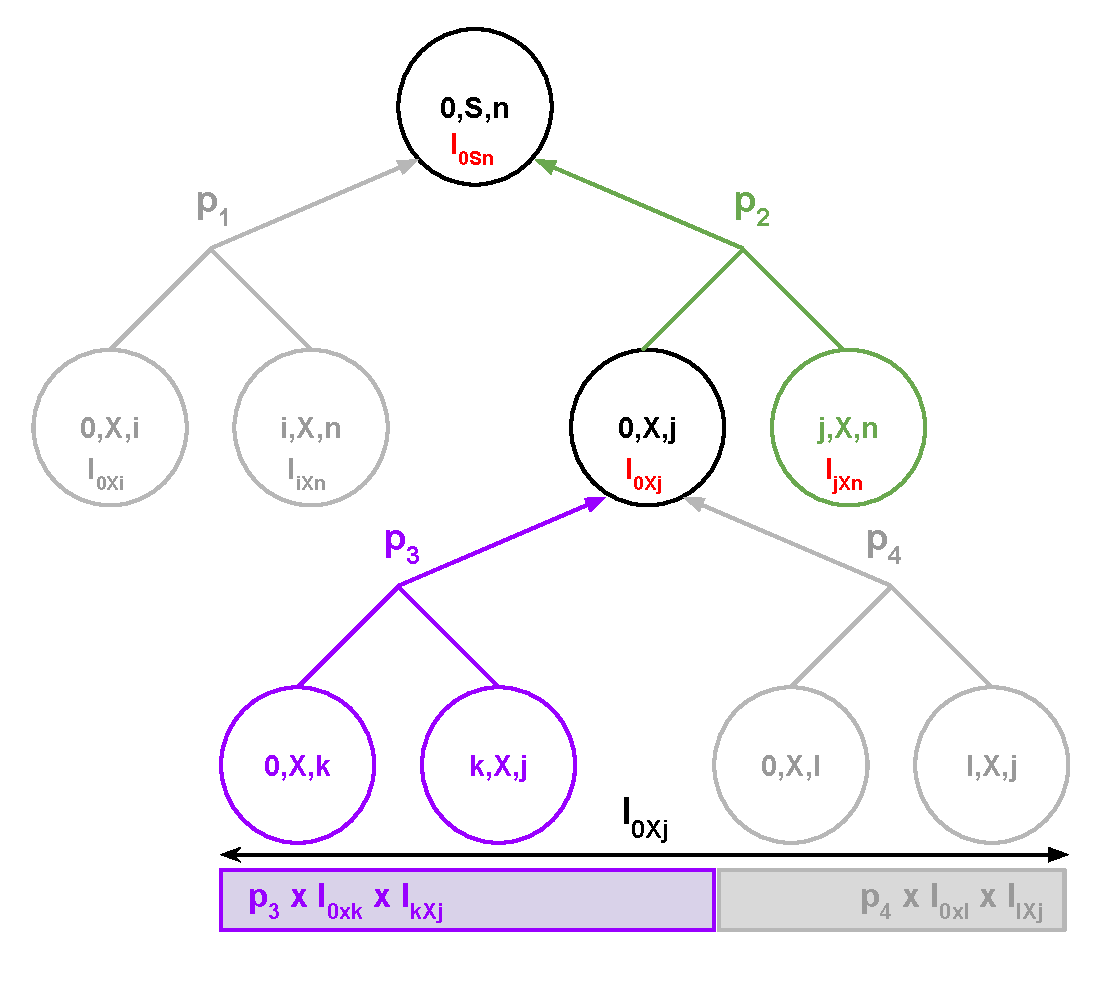
\includegraphics[scale=0.3]{img/viterbi6}
	}
}

\frame{

	Use Inside computed in the Sum-Times semiring!
	
	\frametitle{Sampling}
	\only<1>{
	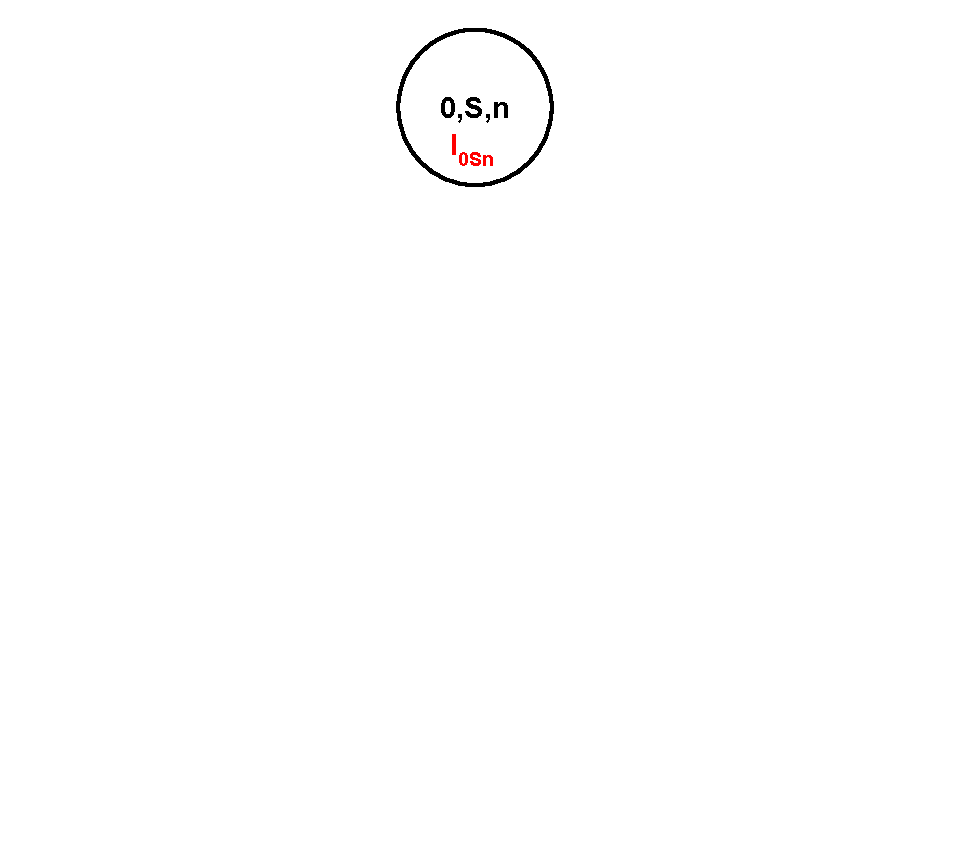
\includegraphics[scale=0.3]{img/sampling0}
	}
	\only<2>{
	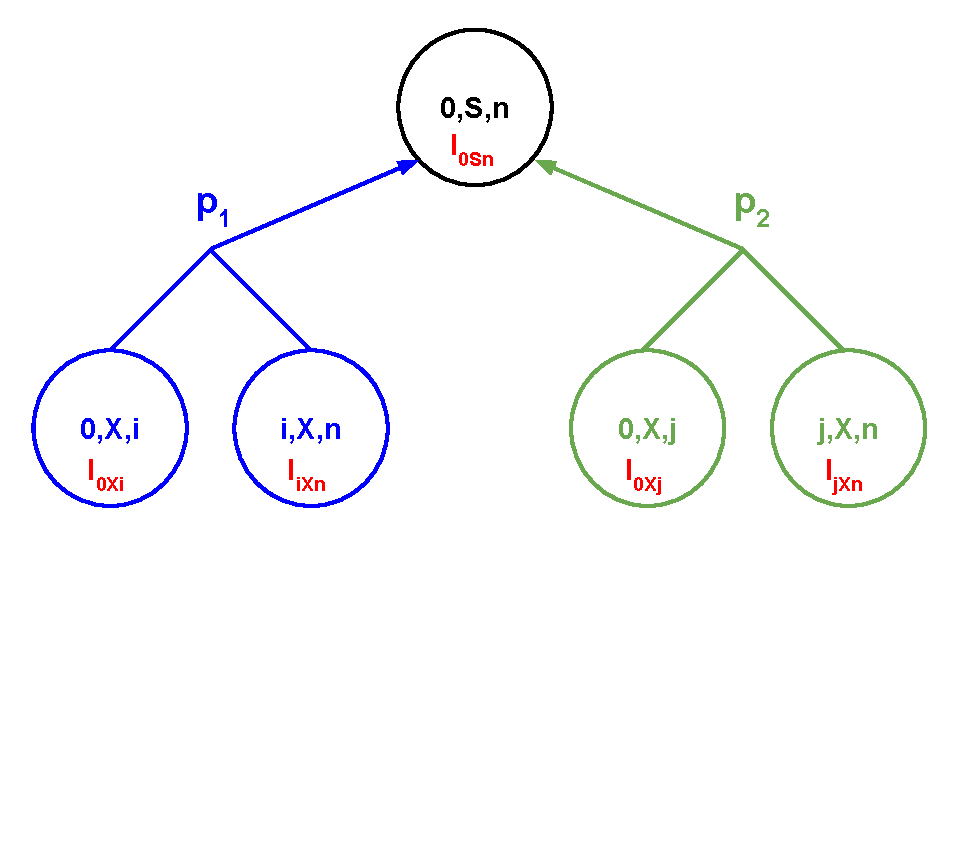
\includegraphics[scale=0.3]{img/sampling1}
	}
	\only<3>{
	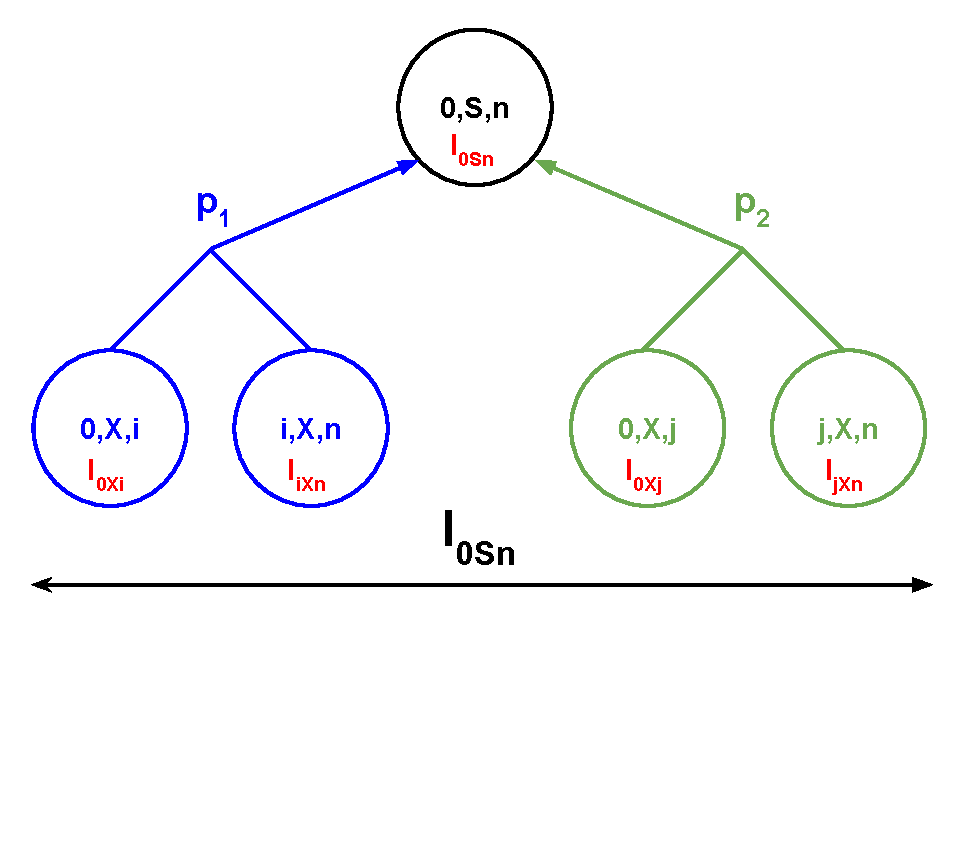
\includegraphics[scale=0.3]{img/sampling2}
	}
	\only<4>{
	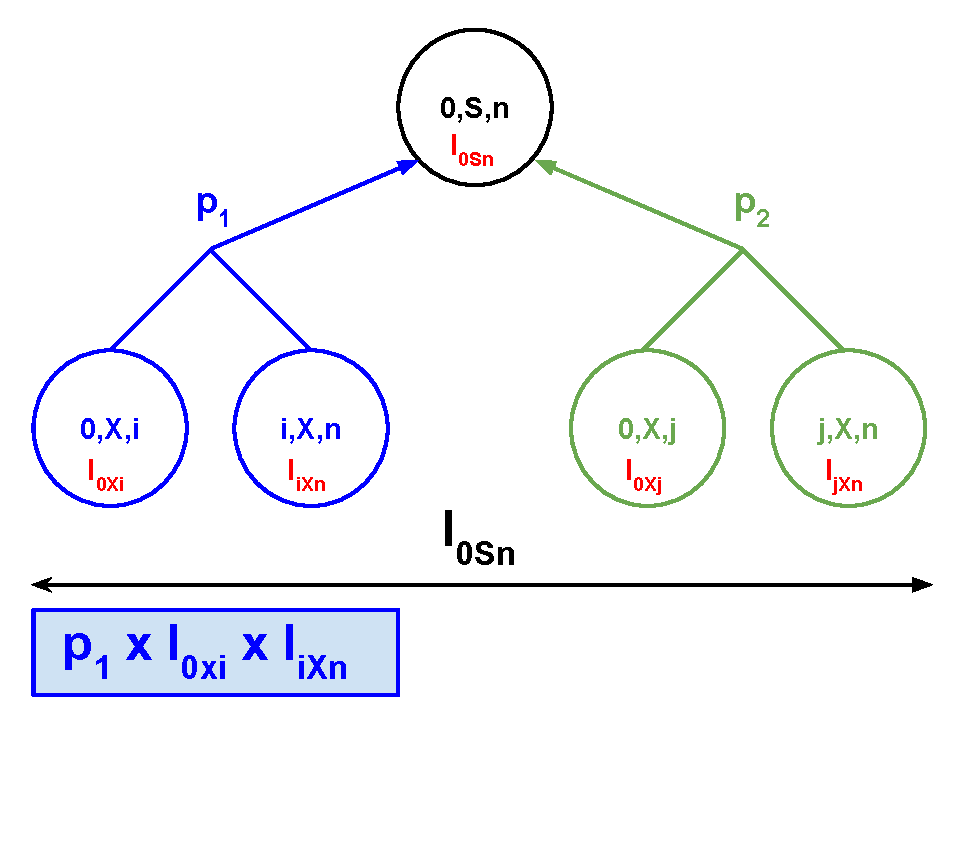
\includegraphics[scale=0.3]{img/sampling3}
	}
	\only<5>{
	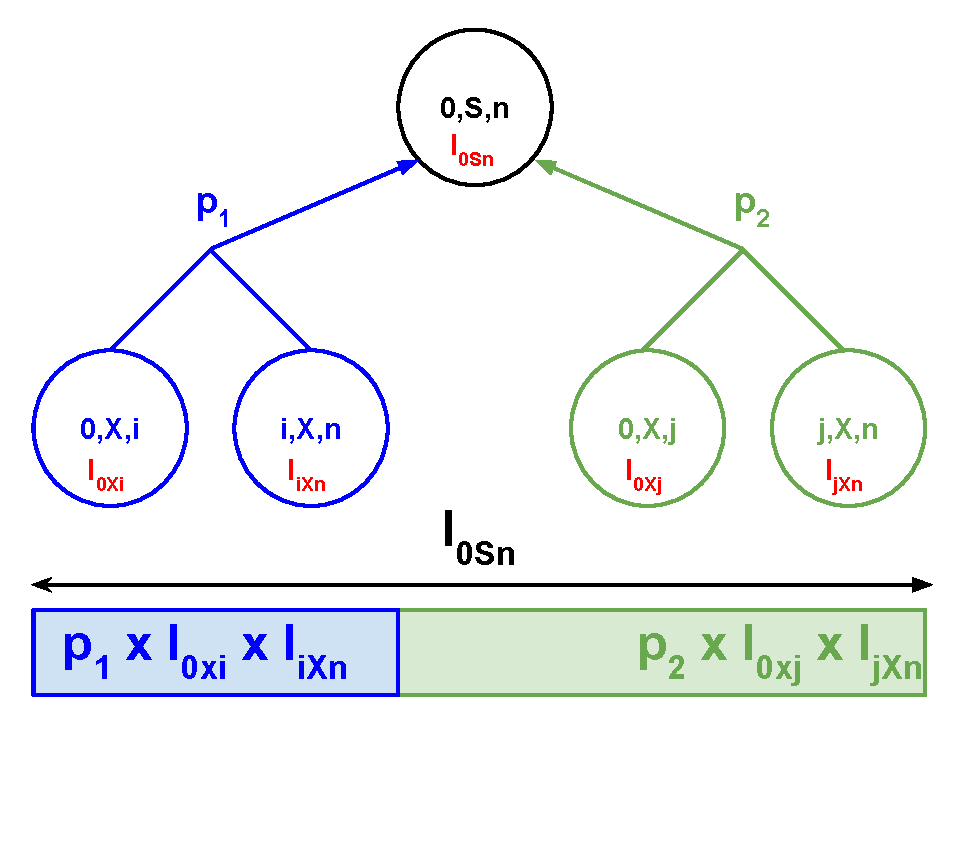
\includegraphics[scale=0.3]{img/sampling4}
	}
	\only<6>{
	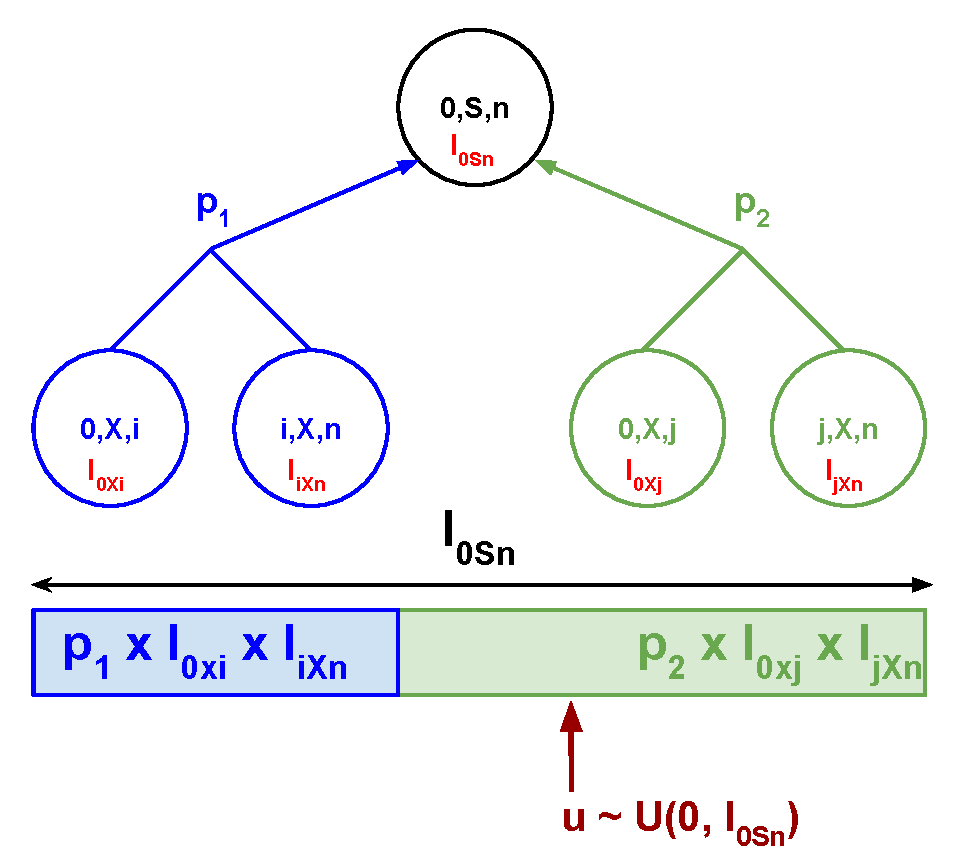
\includegraphics[scale=0.3]{img/sampling5}
	}
	\only<7>{
	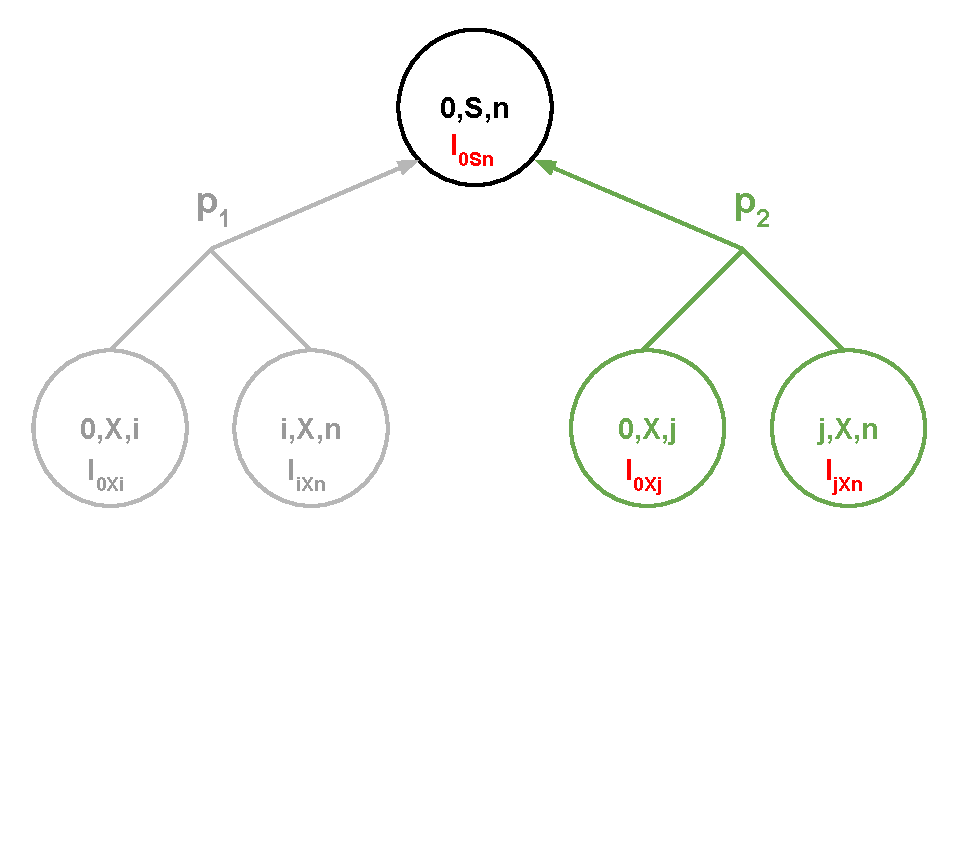
\includegraphics[scale=0.3]{img/sampling6}
	}
	\only<8>{
	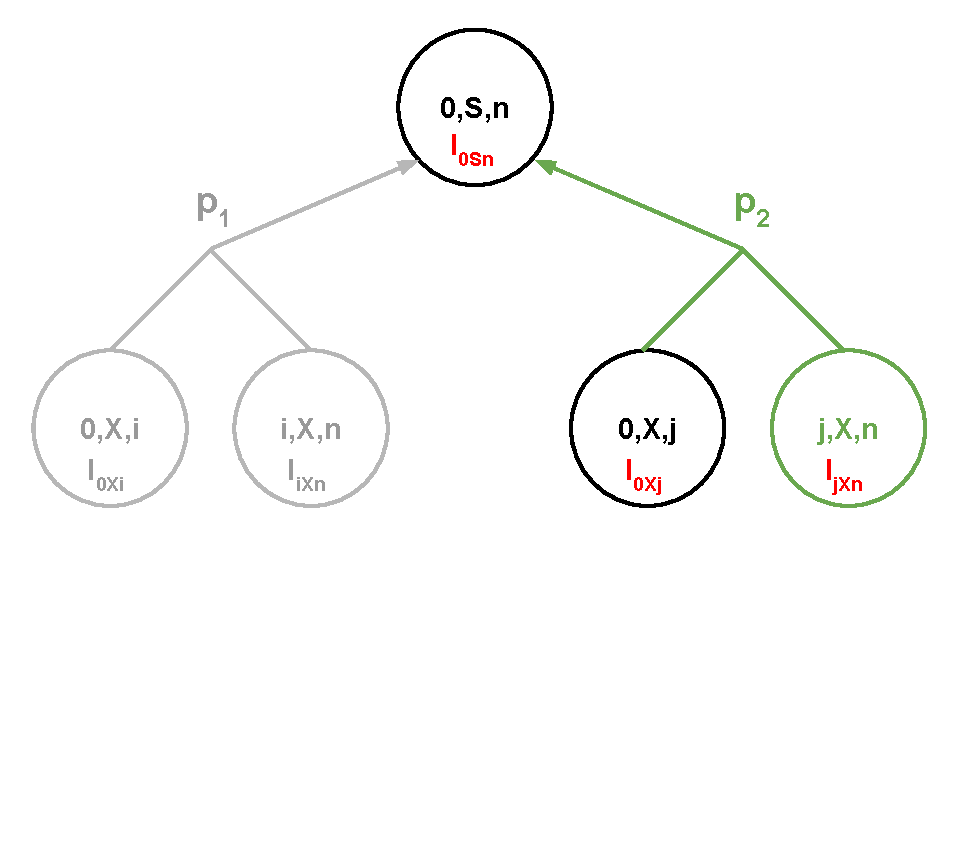
\includegraphics[scale=0.3]{img/sampling7}
	}
	\only<9>{
	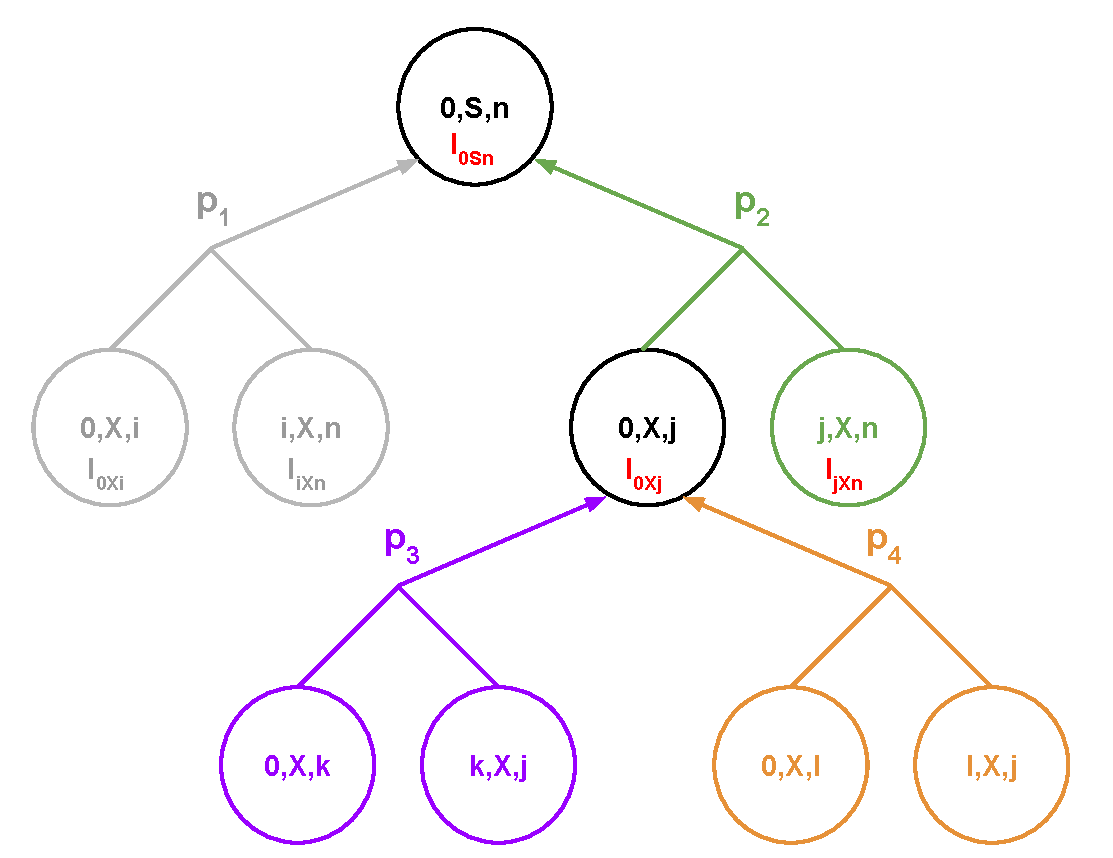
\includegraphics[scale=0.3]{img/sampling8}
	}
	\only<10>{
	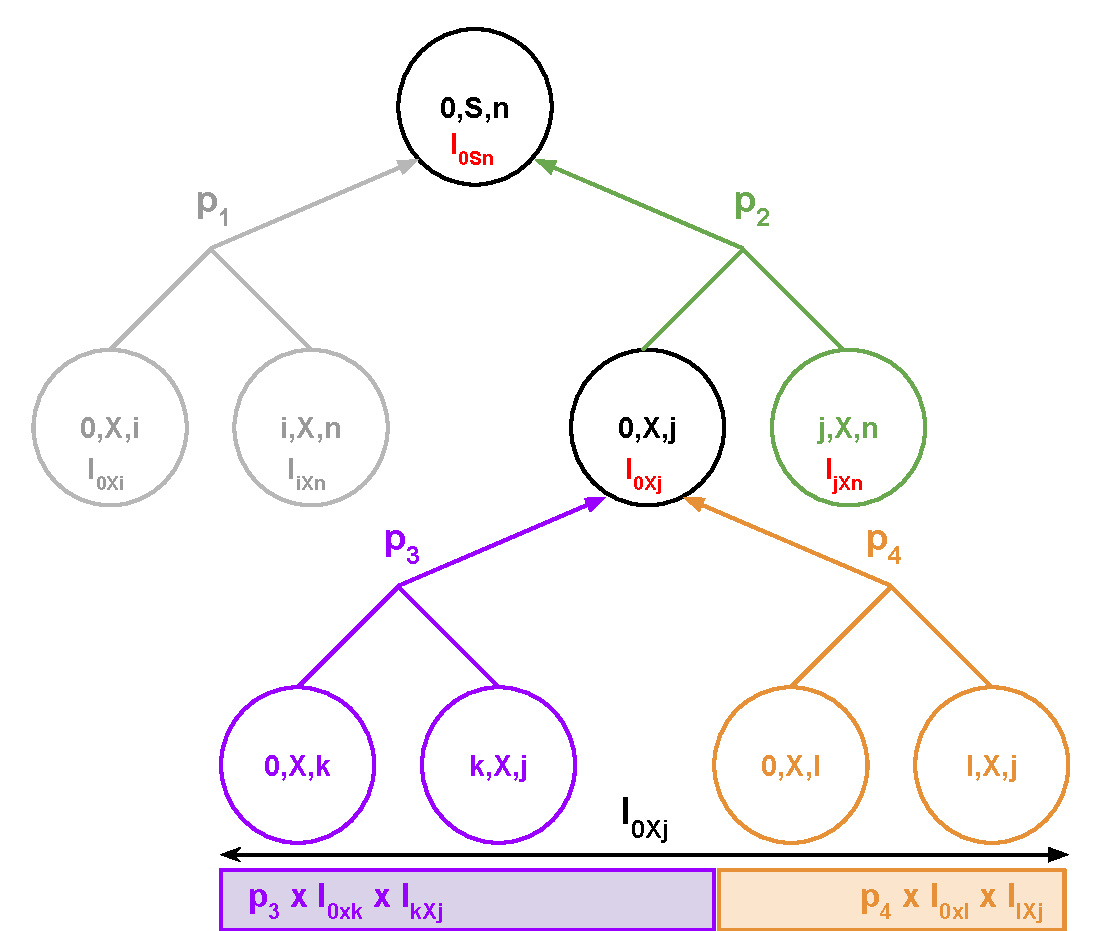
\includegraphics[scale=0.3]{img/sampling9}
	}
	\only<11>{
	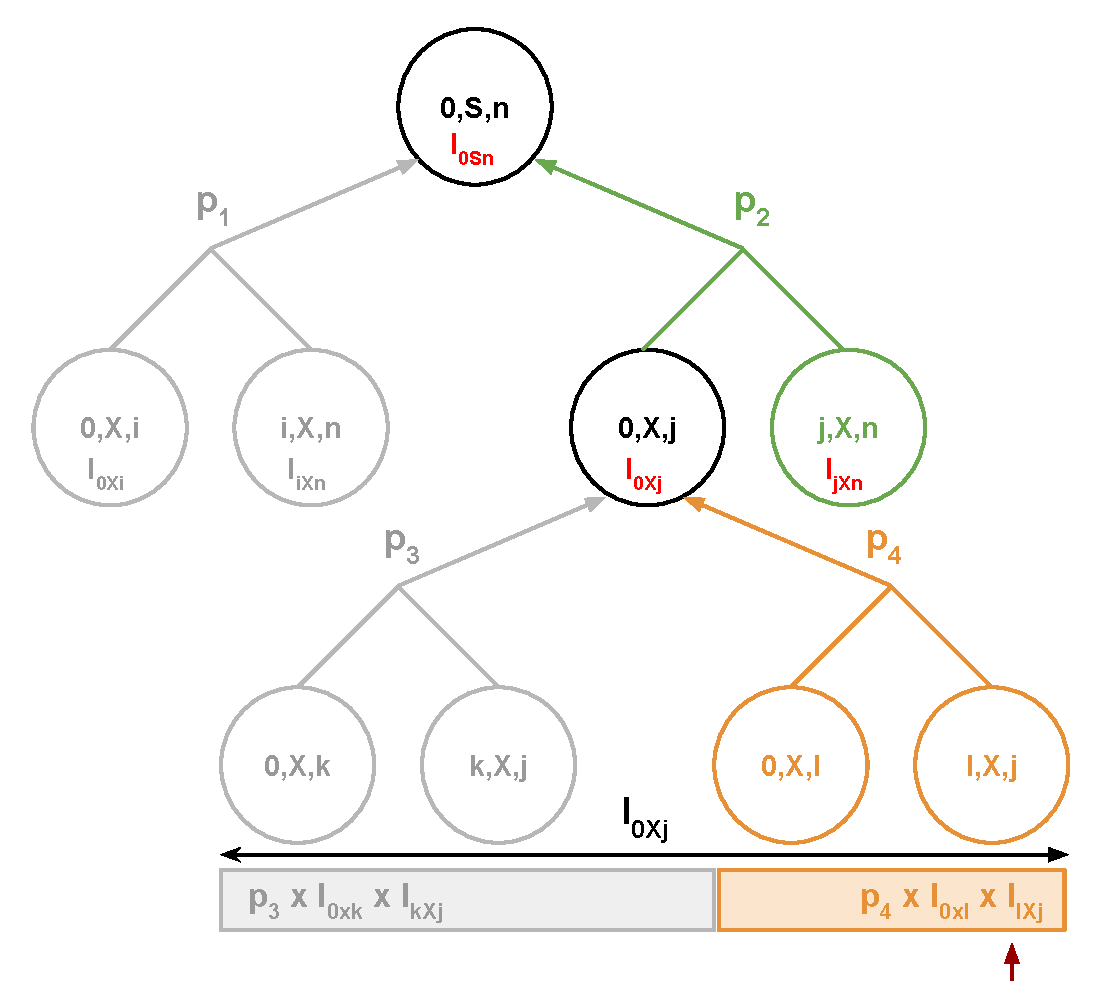
\includegraphics[scale=0.3]{img/sampling10}
	}



}

